\chapter{Classical geometry}
% TODO Classical geometry missing concepts
% proof these using euclidian geometry
% - circle area http://www.ugrad.math.ubc.ca/coursedoc/math101/notes/integration/archimedes.html
% - http://math.furman.edu/~jpoole/euclidselements/eubk3/props.htm
% Lines (goes on idefinetky in bith directiins)
% - Paraell lines
% - rays (has one end point and continjes forever in one direcyion))
% - segments (has start and end)
% - perpendicular
% Postulates
% Circle
% - circumference of a circle 2 \cdot \pi \cdot r = \pi \cdor d
% - area of a circle \pi \cdot r^2 
% perimeter, area, volume (relation to meassure)
% proof thales intercept theorem
% angels (degrees)
% + Radians versious degrees (conversion between the two)
% - corosponding
% - acute < 90
% - obtuse > 90
% - riggt = 90
% - orthogonal
% - vertex (The point about which an angle is measured)
% - adjacent = Two angles are Adjacent when they have a common side and a common vertex (corner point) and don't overlap.
% - supplementary =
% - complementary =
% - vertical =
% Semilar figures
% Triangles
% - Similar triangles
% - Area of triangles
% - Triangle altitude
% - Acute triangle (triangle with all angles below 90)
% - Obtuse triangle (triangle with one angle above 90)
% - Equilateral triangle (a triangle in which all three sides are equal)
% - Scalene triangle (a triangle that has three unequal sides)
% - Isosceles triangle (a triangle with (at least) two equal sides)
% - Area = h*b/2
% - proof any side of a triangle ia always shorter than the sum of the two others
% Polygon
% Quadrilateral (including which contains each other (a square is a retangle and a rhombus)
% - Rhombus (paralellogram with sides of same length)
% - Square
% - Rectangle
% - paralellogram (inckuding area)
% - Trapezoid (A quadrilateral with at least one pair parallel sides.)
% solids
% - pyramid, prism, cone, sphere and cube
% Length
% - mm, cm, dm, km
% - 1 foot = 12 inches
% - 1 yard = 3 feet = 36 inches
% - 1 mile = 1,760 yards = 5,280 feet = 63,360 inches
% Volume
% - mili, centi, deci
% - 1 quart = 2 pints = 4 cups = 32 fluid ounces
% - 1 gallon = 4 quarts = 8 pints = 16 cups = 128 fluid ounces
% Mass
% - mg, kg, ton
% - 1 pound = 16 ounces, 1 ton = 2000 pound
% Figure decomposition (fx calculatijf the are of a trapez by viewing it as a sqare and some triangles)
% -  slices : A horizontal slice through a three-dimensional solid produces a two-dimensional shape.

Geometry arrose as practical methods in the ancient world in order to measure land, survey fields, compute the quantity of corn in containers, and to construct temples and pyramids. The theorems of Thales and Pythagoras, which are the oldest theorems of humanity and fundamental tools for geometry.

Later these methods practiced by builders and tradesmen where taken over by Euclid who replaced the geometry of nails, ropes and walls used by the temple builders with mathematical points, lines, rectangles etc., objects of pure reasoning, which require a list of definitions, \index{axiom}s and \index{postulate}. This is the origin of nearly all mathematical procedures used ever since.

\section{Classical plane geometry}
The most beautiful and useful discoveries in classical geometry concerns the relations between lengths (Thales’ intercept theorem), angles (the central angle theorem of Euclid) areas (the Pythagorean theorem).

\subsection{Thales theorem}
Thales is the man to tell us how to measure the height of a tree without having to climb it. In figure \ref{geo:thales} below we let side $B'C'$ be the height of the tree and $AB'$ be its shadow. We erect a vertical stick $BC$ in such a manner that $AB$ is the shadow of the stick. We then measure the distance $AB$, say $4$ metres, the distance $AB'$, say $8$ metres, and the stick $BC$, say $5$ metres. By parallel displacements of the triangle $ABC$ we see that, since $AB′$ measures twice $AB$, the height $B'C'$ will measure twice $BC$, hence $B'C' = 2 \cdot 5 = 10$.
\begin{figure}[H]
\label{geo:thales}
\centering
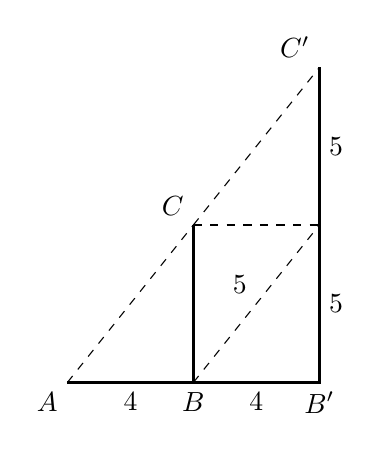
\begin{tikzpicture}
    % constants
    \def\trigwidth{1.6cm}
    \def\trigheight{2cm}
    % small triangle nodes
    \coordinate [label={below left:$A$}]   (A) at (0, 0);
    \coordinate [label={below:$B$}]  (B) at (\trigwidth, 0);
    \coordinate [label={above left:$C$}]  (C) at (\trigwidth, \trigheight);
    % large triangle nodes
    \coordinate [label={below:$B'$}] (B') at (2*\trigwidth, 0);
    \coordinate [label={above left:$C'$}] (C') at (2*\trigwidth, 2*\trigheight);
    \coordinate (B'C'mid) at (2*\trigwidth, \trigheight);
    % lengths labels
    \coordinate [label={below:$4$}] (ABmid) at (0.5*\trigwidth, 0);
    \coordinate [label={below:$4$}] (BB'mid) at (1.5*\trigwidth, 0);
    \coordinate [label={right:$5$}] (x) at (2*\trigwidth, 0.5*\trigheight);
    \coordinate [label={right:$5$}] (y) at (2*\trigwidth, 1.5*\trigheight);
    \coordinate [label={above left:$5$}] (z) at (1.5*\trigwidth, 0.5*\trigheight);
    % small triangle
    \draw [very thick] (A) -- (B) -- (C);
    \draw [dashed] (A) -- (C);
    % large triangle
    \draw [very thick] (B) -- (B') -- (C');
    \draw [dashed] (C) -- (C');
    % internal lines
    \draw [dashed] (C) -- (B'C'mid);
    \draw [dashed] (B) -- (B'C'mid);
\end{tikzpicture}
\caption{Using similar triangles to measure the height of a tree}
\end{figure}

\begin{theorem}
(Thales’ intercept theorem). Consider an arbitrary triangle $ABC$ (see figure \ref{geo:similar-triangles} below) and let $AC$  be extended to $C'$ and $AB$ to $B'$ so that $B'C'$ is parallel to $BC$. Then the lengths of the sides satisfy the relations
\[
\frac{a'}{a} = \frac{b'}{b} = \frac{c'}{c}
\textrm{~ and hence ~}
\frac{a'}{c'} = \frac{a}{c},~~
\frac{c'}{b'} = \frac{c}{b},~~
\frac{b'}{a'} = \frac{b}{a}
\]

\end{theorem}
As these proportions are also preserved when the triangle is displaced and rotated we get the following result. \textit{If corresponding angles of two triangles are equal, then corresponding sides are proportional}. Triangles having these properties are called similar (see \index{similarity}).
\begin{figure}[H]
\label{geo:similar-triangles}
\centering
\begin{tikzpicture}[x=0.6cm,y=0.6cm, rotate=10,every node/.style={draw}]
    % constants
    \def\aLength{3}
    \def\bLength{4}
    \def\cLength{5}
    \def\amLength{6}
    \def\bmLength{8}
    \def\cmLength{10}
    % small triangle nodes
    \coordinate [label={below left:$A$}] (A) at (0, 0);
    \coordinate [label={below:$B$}] (B) at (\cLength, 0);
    \coordinate [label={above left:$C$}] (C) at (\cLength, \aLength);
    % large triangle nodes
    \coordinate [label={below right:$B'$}] (B') at (\cmLength, 0);
    \coordinate [label={above right:$C'$}] (C') at (\cmLength, \amLength);
    % length labels
    \coordinate [label={right:$a$}] (a) at (\cLength, 0.5*\aLength);
    \coordinate [label={above:$b$}] (b) at (0.5*\bLength, 0.5*\aLength);
    \coordinate [label={below:$c$}] (c) at (0.5*\cLength, 0);
    \coordinate [label={right:$a'$}] (a') at (\cmLength, 0.5*\amLength);
    \coordinate [label={above right:$b'$}] (b') at (0.5*\bmLength, 0.5*\amLength+0.75);
    \coordinate [label={below:$c'$}] (c') at (0.5*\cmLength, -0.75);
    % angel labels

    % small triangle
    \draw [very thick] (A) -- (C) -- (B) -- (A);
    % large triangle
    \draw [dashed] (B) -- (B') -- (C') -- (C);
\end{tikzpicture}
\caption{Similar triangles}
\end{figure}

\subsection{Points, Lines and Planes}

\subsection{Angles}

\subsubsection{Radians}
% TODO draw radian drawing
Degrees are often used when introducting geometry. However for more advanced  work we often meassure angles in radians. Radians equals the ratio between the length of an angle arc and its radius. As the circumference of a circle equals $2\pi r$ thus an angle of $360 deg$ equals $\frac{2\pi r}{r} = 2\pi$ radians. Radians allow us to use real numbers in the trigonometric functions, rather than degrees, which are an arbitrary angular measurement between $0-360$. The use of real numbers for meassuring angels allow is essential in more advanced mathematics, calculus for example.

\section{Area and perimeter}
The area of a parallelogram is $a \cdot h$, where h is the altitude of the parallelogram (Eucl. I.35). There are two ways to see this: (a) We cut off the triangle on the left and add it on the right to obtain a rectangle (Euclid’s proof, see the second figure in Fig. 1.11); (b) We cut the parallelogram parallel to AB into a large number of very slim rectangles. The area of a triangle is half the area of the parallelogram.

\subsection{Triangles}
Figure 1.2 shows a right-angled triangle (ie a triangle with one angle of 90°) with another angle denoted by the Greek letter theta θ. The sides of the a right-angled triangle are called the adjacent side (next to θ), the opposite side (opposite to θ) and the hypotenuse (opposite the right-angle).

\subsection{Circle}
\begin{figure}[H]
\begin{tikzpicture}[scale=1.5]
    \tkzDefPoint(0,0){O}
    \tkzDefPoint(1,1){B}
    \tkzDefPoint(0.55,0.45){R}
    \tkzDefPoint(1,0.99){A}
    \tkzDrawArc(O,B)(A)
    \tkzDrawLines[add = 0 and 0](O,A)
    \tkzDrawPoints(O,B)
    \tkzLabelPoints[below](O,R)
    \tkzLabelPoints[right](B)
\end{tikzpicture}
\end{figure}
\noindent The area of a circle is
\begin{equation}
A = \pi \cdot r^2
\end{equation}
the perimeter (circumference) is
\begin{equation}
C = 2\pi \cdot r
\end{equation}

\section{Euclid Elements}
He begins with some definitions of the basic concepts: point, line, circle, triangle, quadrilateral. Euclid then states ten axioms (also called postulates)on which all subsequent reasoning is based. We shall note these merely to see that they do indeed describe apparently unquestionable properties of geometric figures. The first five posgulates are:
\begin{enumerate}
    \item Two points determine a unique straight line
    \item A straight line extends indefinitely far in either direction
    \item A circle may be drawn with any given center and any given radius
    \item All right angles are equal
    \item Given a line l ( Fig. 6–1 ) and a point P not on that line, there exists in the plane of P and l and through P one and only one line m , which does not meet the given line l .
\end{enumerate}

% TODO proof - On a given finite straight line AB to construct an equilateral triangle. A B Γ ∆ E The construction is performed by describing a circle∆centred at A and passing through B (Post. 3) and another circle E centred at B and passing through A (Post. 3). Their point of intersectionΓis then joined to A and to B (Post. 1). The distance AΓis equal to BΓand to AB, which makes the triangle equilateral.

% TODO proof Eucl. I.4, I.8, VI.2 (TODO is this thales theorem)

% TODO proof - The sum of the three angles of an arbitrary triangle ABC is equal to two right angles:

% TODO interestinf geometric things to proof
% - angles of triqngles, quadrilaterals and circles
% - area/of triangles and quadrilaterals 
% - pythagoras (move proof from geometry history book)
% - Squaring the circle. Finding a square whose area is equal to that of a given rectangle
% - Doubling the cube. The problem is:find a cube whose volume is twice that of a given cube
% - Trisecting an angle.
% - Find (all) right-angled triangles with all sides (TODO proof that no more exists)

Adding four right-angled triangles with sides a and b, we arrive at and get the large square of area $(a + b)^2 = a 2 + 2ab + b 2$ . Since the areas of the four triangles add up to $2ab$, the square with area $c^2$ also has area $a^2 + b^2$. 

% TODO proof - An exterior angle of a triangle is greater than either remote interior angle of the triangle.


\section{Classical solid geometry}
\subsection{Cube}
\subsection{Cone}
\subsection{Sphere}

\section{Trigonometry}
% TODO Pythagorean trigonometric identity

\section{Exercises}
\begin{ExerciseList}

% TODO 
% - area calculation excericses (amount of tiles 0.25m^2 tiles needed to cover 15m^2
% - compare area and peremter of squares
% - using thales theorem

\end{ExerciseList}
